% LaTeX source for ``การเรียนรู้ของเครื่องสำหรับเคมีควอนตัม (Machine Learning for Quantum Chemistry)''
% Copyright (c) 2022 รังสิมันต์ เกษแก้ว (Rangsiman Ketkaew).

% License: Creative Commons Attribution-NonCommercial-NoDerivatives 4.0 International (CC BY-NC-ND 4.0)
% https://creativecommons.org/licenses/by-nc-nd/4.0/

\chapter{การเรียนรู้แบบไม่มีผู้สอน}
\label{ch:unsup_ml}

การเรียนรู้แบบไม่มีผู้สอน (Unsupervised Learning) เป็นเทคนิคที่อาจจะเรียกว่าได้ตรงข้ามกับการเรียนรู้แบบมีผู้สอน (Supervised Learning) 
ก็ได้ เพราะว่าเทคนิคประเภทนี้จะเป็นการฝึกสอนโมเดลแบบไม่มีการบอกคำตอบหรือเอาต์พุตให้โมเดลได้รับรู้ ดังนั้นสิ่งที่โมเดลมีอย่างเดียวก็คืออินพุต
ซึ่งสิ่งเดียวที่โมเดลจะทำได้นั่นก็คือการเรียนรู้หาความสัมพันธ์ (Relation) ระหว่างข้อมูลแต่ละตัวภายในชุดข้อมูลที่เราได้ป้อนเข้าไป 
การเรียนรู้ประเภทนี้จะพิจารณาข้อมูลเป็นเซตของตัวแปรสุ่ม แล้วจึงสร้างโมเดลความหนาแน่นร่วมของชุดข้อมูล การเรียนรู้แบบไม่มีผู้สอนสามารถนำไปใช้%
ร่วมกับการทฤษฎีของเบย์ (Bayes' theorem) เพื่อหาความน่าจะเป็นแบบมีเงื่อนไขของตัวแปรสุ่มโดยกำหนดตัวแปรที่เกี่ยวข้องให้ 
นอกจากนี้ยังสามารถนำไปใช้ในการบีบอัดข้อมูล (Data Compression) ซึ่งขั้นตอนวิธีการบีบอัดข้อมูลจะขึ้นอยู่กับการแจกแจงความน่าจะเป็นของข้อมูล

จริง ๆ แล้วการเรียนรู้แบบไม่มีผู้สอนนั้นมีเทคนิคย่อยต่าง ๆ มากมาย เพื่อไม่ให้สับสน ในบทนี้ผู้เขียนจะขอจัดกลุ่มอัลกอริทึม Unsupervised ML ดังนี้

\begin{itemize}
    \item การวิเคราะห์การจัดกลุ่ม Clustering Analysis
    \item การลดจำนวนมิติของข้อมูลแบบเชิงเส้น (Linear Dimensionality Reduction)
    \item การลดจำนวนมิติของข้อมูลแบบไม่เชิงเส้น (Nonlinear Dimensionality Reduction)
\end{itemize}

%--------------------------
\section{วิธีการจัดกลุ่ม}
\label{sec:clustering}
\idxboth{การวิเคราะห์การจัดกลุ่ม}{Clustering Analysis}
\idxboth{วิธีการจัดกลุ่ม}{Clustering}
%--------------------------

เทคนิคการวิเคราะห์การจัดกลุ่ม (Clustering Analysis) หรือจะเรียกสั้น ๆ ว่า Clustering ก็ได้ มีเทคนิคย่อยอีกมากมายที่ถูกนำมาใช้อย่าง%
แพร่หลายในการวิเคราะห์ข้อมูลทางเคมี

นอกจากนี้ สิ่งที่หลายคนมักจะสับสนและเข้าใจผิดก็คือ Clustering กับ Classification นั้นเป็นสิ่งเดียวกัน ซึ่งจริง ๆ แล้วไม่ใช่ โดยทั้งสองวิธีนี้%
มีความแตกต่างกันดังนี้

\begin{description}
    \item[\textbf{Clustering}] ชุดข้อมูลไม่มีการถูกแบ่งกลุ่มมาก่อน (Unlabelled) มีเพียงเเค่ข้อมูลมาให้ โดย Clustering 
    ยังสามารถแบ่งออกได้เป็นสองแบบ ดังนี้
    \idxen{Clustering!Hard Clustering}
    \idxen{Clustering!Soft Clustering}
    \begin{itemize}
        \item Hard Clustering เป็นการกำหนดให้แต่ละชุดข้อมูลแบ่งออกเป็นกลุ่มที่แยกออกจากกันโดยสิ้นเชิง
        \item Soft Clustering เป็นการที่ข้อมูลมีโอกาสที่จะอยู่ในหลาย ๆ กลุ่มได้ ขึ้นอยู่กับความน่าจะเป็นของตัวข้อมูล
    \end{itemize}
    \item[\textbf{Classification}] ชุดข้อมูยนั้นมีการแบ่งกลุ่มมาแล้ว (Labelled) โดยรู้จำนวนของกลุ่มและรู้ว่ามีการแบ่งกลุ่มอย่างไร
\end{description}

\begin{figure}[H]
    \centering
    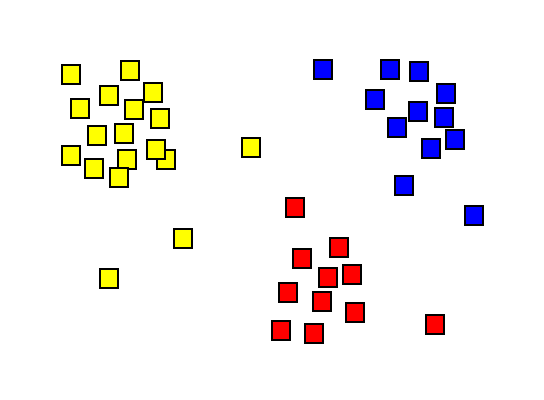
\includegraphics[width=0.8\linewidth]{fig/cluster.png}
    \caption{ตัวอย่างของชุดข้อมูลที่ถูกจัดกลุ่มโดยแบ่งตามสี}
    \label{fig:cluster}
\end{figure}

เทคนิค Clustering นั้นเป็นการจัดกลุ่มข้อมูลที่ไม่เคยมีการจัดกลุ่มมาก่อน กล่าวคือถ้าหากเรามีชุดข้อมูลที่ไม่เคยถูกวิเคราะห์ก่อนซึ่งข้อมูลเหล่านั้นก็%
ผสมกันแบบมั่ว ๆ หรือไม่มีรูปแบบ เราสามารถแบ่งกลุ่มข้อมูลได้โดยพิจารณาจากลักษณะที่คล้ายกันของข้อมูล โดยจะนำข้อมูลที่มีลักษณะคล้ายกัน%
มาอยู่กลุ่มเดียวกัน ส่วนข้อมูลที่มีลักษณะต่างออกไปก็ให้ไปอยู่อีกกลุ่มหนึ่ง การนำเทคนิคนี้ไปใช้คือจะไม่ใช่การหาผลลัพธ์ที่ต้องการวัดค่าความแม่นยำ 
แต่จะเป็นการหาความสัมพันธ์ของข้อมูลอีกรูปแบบหนึ่ง เช่น การจัดกลุ่มข้อมูลของสารประกอบเคมีอินทรีย์จากความว่องไว้ในการเข้าทำปฏิกิริยา 
การจัดกลุ่มหมู่ฟังก์ชันจากชนิดของการเข้าทำปฏิกิริยา

%--------------------------
\subsection{การจัดกลุ่มแบบโครงสร้างลำดับชั้น}
\label{ssec:hierar_clustering}
\idxboth{การจัดกลุ่มแบบโครงสร้างลำดับชั้น}{Hierarchical Clustering}
%--------------------------

การจัดกลุ่มแบบโครงสร้างลำดับชั้นจะใช้ลักษณะของต้นไม้ในการแทนความเชื่อมโยงของข้อมูล เป็นเทคนิคที่เหมาะสำหรับข้อมูลที่มีลำดับชั้น เช่น 
อนุกรมวิธาน (Taxonomy) การแบ่งกลุ่มลักษณะนี้มี 2 ประเภท คือ ล่างขึ้นบน (Agglomerative) และ บนลงล่าง (Divisive) ดังนี้ 

\begin{itemize}
    \item Agglomerative ในขั้นตอนแรกข้อมูลแต่ละตัวในชุดข้อมูลนั้นนับเป็นหนึ่งกลุ่ม หลังจากนั้นทำการคำนวณหาค่าความใกล้ชิดของกลุ่มที่อยู่%
    ใกล้กัน ซึ่งกลุ่มที่อยู่ใกล้กันก็จะถูกรวบกันเป็นหนึ่งกลุ่ม โดยวนทำเช่นนี้ไปเรื่อย ๆ จนกว่าจะได้กลุ่มข้อมูลเดียวในที่สุด
    \item Divisive เทคนิคนี้จะดำเนินการตรงกันข้ามกับ Agglomerative ในขั้นตอนแรกเริ่มจากกลุ่มใหญ่กลุ่มเดียว และแยกกลุ่มที่ไม่เหมือนกัน%
    ออกไปเรื่อย ๆ จนกระทั่งได้จำนวนกลุ่มเท่ากับจำนวนข้อมูลหรือจนกว่าจะแยกต่อไม่ได้ 
\end{itemize}

นอกจากนี้ยังมีเทคนิคการจัดกลุ่มข้อมูลแบบอื่นอีกที่ไม่ได้กล่าวถึง เช่น Centroid-based Clustering ใช้จุดกึ่งกลางของกลุ่ม, Density-based 
Clustering ใช้ความหนาแน่นหรือความแออัดของข้อมูล และ Distribution-based Clustering ใช้รูปแบบการแจกแจงของข้อมูล

%--------------------------
\subsection{วิธีรวบกลุ่มจับคู่แบบถ่วงน้ำหนักโดยใช้ค่าเฉลี่ยเลขคณิต}
\label{ssec:wpgma}
\idxboth{วิธีรวบกลุ่มจับคู่แบบถ่วงน้ำหนักโดยใช้ค่าเฉลี่ยเลขคณิต}{Weighted Pair Group Method with Arithmetic Mean}
%--------------------------

วิธีรวบกลุ่มจับคู่แบบถ่วงน้ำหนักโดยใช้ค่าเฉลี่ยเลขคณิต (Weighted Pair Group Method with Arithmetic Mean หรือ WPGMA) 
เป็นเทคนิคการจัดกลุ่ม (Clustering) แบบหนึ่งของวิธีโครงสร้างลำดับชั้น (Hierarchical Method) ซึ่งพัฒนาขึ้นมาโดยใช้ Pairwise 
Similarity Matrix\autocite{sokal1958} โดยนักชีววิทยาเชิงสถิติ Robert Reuven Sokal และนักกีฏวิทยา Robert Reuven Sokal

%--------------------------
\section{การแบ่งกลุ่มข้อมูลแบบเคมีน}
\label{sec:k_means}
\idxen{K-means Clustering}
%--------------------------

การแบ่งกลุ่มข้อมูลแบบเคมีน (K-means Clustering) เป็นหนึ่งในวิธีการแบ่งเวกเตอร์ซึ่งจะเป็นการแบ่งชุดข้อมูลที่มี n ข้อมูลออกเป็น k กลุ่ม
ซึ่งเทคนิคนี้ได้ถูกใช้มาอย่างยาวนานตั้งแต่ในช่วงยุคเริ่มต้นของการทำ Data Mining\autocite{macqueen1967}

\begin{figure}[H]
    \centering
    \begin{subfigure}{0.5\textwidth}
        \centering
        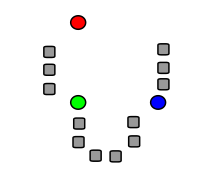
\includegraphics[width=0.9\linewidth]{fig/k-means-step1.png}
        \caption{เลือกค่าเฉลี่ย}
        \label{fig:k_means_step1}
    \end{subfigure}%
    \begin{subfigure}{0.5\textwidth}
        \centering
        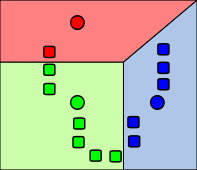
\includegraphics[width=0.9\linewidth]{fig/k-means-step2.png}
        \caption{สร้างคลัสเตอร์ k กลุ่ม}
        \label{fig:k_means_step2}
    \end{subfigure}
    \\
    \vspace{1em}
    \begin{subfigure}{0.5\textwidth}
        \centering
        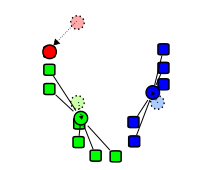
\includegraphics[width=0.9\linewidth]{fig/k-means-step3.png}
        \caption{คำนวณค่าเฉลี่ยใหม่}
        \label{fig:k_means_step3}
    \end{subfigure}%
    \begin{subfigure}{0.5\textwidth}
        \centering
        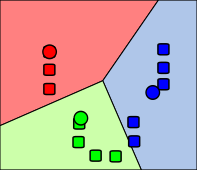
\includegraphics[width=0.9\linewidth]{fig/k-means-step4.png}
        \caption{ทำซ้ำจนกระทั่งค่ากลางลู่เข้า}
        \label{fig:k_means_step4}
    \end{subfigure}
    \caption{ขั้นตอนการทำ K-means Clustering (เครดิตภาพ: \url{https://en.wikipedia.org/wiki/K-means_clustering})}
    \label{fig:k_means}
\end{figure}
 
ภาพที่ \ref{fig:k_means} แสดงอัลกอริทึมของ K-means Clustering ที่มี 4 ขั้นตอน โดยขั้นตอนที่หนึ่งจะเป็นเลือกค่าเฉลี่ยเริ่มต้น k 
(ในกรณีนี้ k=3) แบบสุ่มจากโดเมนข้อมูล ขั้นตอนที่สองเป็นการสร้างคลัสเตอร์ k กลุ่มรอบ ๆ ค่าเฉลี่ยทีได้กำหนดไว้โดยการเชื่อมโยงทุกข้อมูล%
การสังเกตด้วยค่าเฉลี่ยที่ใกล้ที่สุด (สังเกตระยะห่างระหว่างจุดวงกลมในแต่ละคลัสเตอร์ไปจนถึงเส้นแบ่ง) เส้นแบ่งในที่นี้แสดงให้เห็นแผนภาพของโวโรนอย 
(Voronoi Diagram) ที่สร้างขึ้นจากค่าเฉลี่ย ขั้นตอนที่สามคือคำนวณจุดศูนย์กลางหรือจุดเซนทรอยด์ (Centroid) ของโวโรนอยของแต่ละคลัสเตอร์%
และทำการกำหนดเป็นค่าเฉลี่ยค่าใหม่ ขั้นตอนที่สี่จะเป็นการทำสามขั้นตอนแรกซ้ำ ซึ่งจะทำซ้ำไปเรื่อย ๆ จนกว่าค่ากลางของแต่ละคลัสเตอร์จะไม่เปลี่ยนแปลง
โดยเมื่อค่ากลางลู่เข้าแล้ว เราจะได้ฟังก์ชันที่มีเส้นแบ่งสำหรับการนำไปจัดคลัสเตอร์ของข้อมูล Test Set ต่อไป

ลำดับต่อไปคือวิธีการลดขนาดมิติของข้อมูลแบบเชิงเส้นซึ่งผู้เขียนขออธิบาย 2 วิธี คือ

\begin{itemize}
    \item Principal Component Analysis (PCA)
    \item Multidimensional Scaling (MDS)
\end{itemize}

%--------------------------
\section{การวิเคราะห์องค์ประกอบหลัก}
\label{sec:pca}
\idxboth{การวิเคราะห์องค์ประกอบหลัก}{Principal Component Analysis}
%--------------------------

\begin{figure}[H]
    \centering
    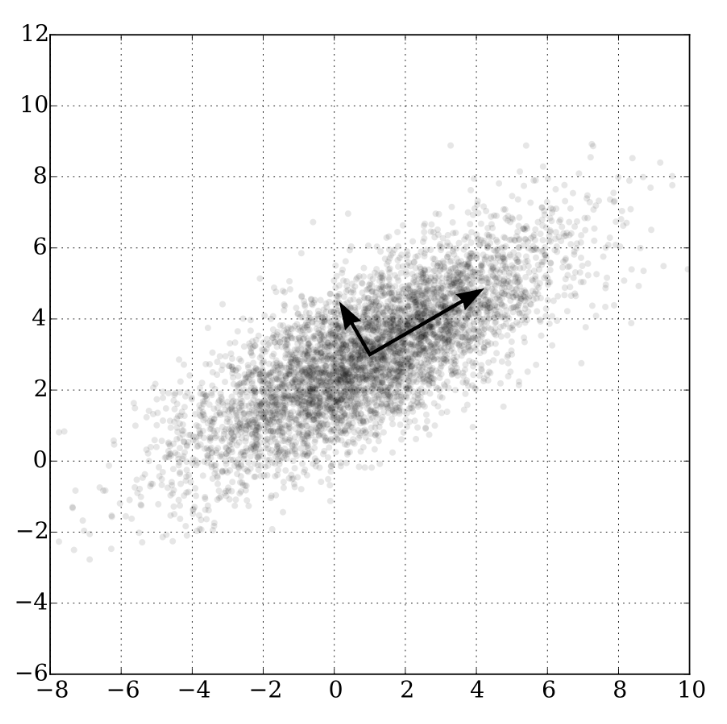
\includegraphics[width=0.8\linewidth]{fig/pca.png}
    \caption{Principal Component Analysis ของข้อมูลที่มีการกระจายตัวแบบเกาส์เซียนหลายตัวแปร (Multivariate Gaussian
    Distribution) เวกเตอร์ที่แสดงนั้นเป็น Eigenvector ของ Covariance Matrix ที่มีการปรับขนาด (Scaled) โดยใช้ค่ายกกำลังสองของ 
    Eigenvalue และมีการปรับตำแหน่งโดยใช้ค่าเฉลี่ย}
    \label{fig:pca}
\end{figure}

การวิเคราะห์องค์ประกอบหลัก (Principal Component Analysis หรือ PCA) เป็นวิธีทางสถิติสำหรับการจัดกลุ่มตัวแปร ถูกนำมาใช้เพื่อรับมือกับ%
ข้อมูลที่มีจำนวนหลายมิติหรือมีหลายตัวแปร วิธี PCA ถูกพัฒนาโดยนักคณิคศาสตร์และชีววิทยาเชิงสถิติชาวอังกฤษ Karl Pearson โดยเทคนิค PCA 
สามารถหาความสัมพันธ์ของตัวแปรเหล่านั้นโดยทำการลดขนาดของมิติโดยสร้างชุดข้อมูลใหม่ที่อาศัยแกนอ้างอิงจากชุดข้อมูลเดิม ซึ่งจำนวนมิติที่ถูกลดลง%
นั้นก็มีจำนวนมิติเพียง 2 หรือ 3 มิติเท่านั้น ซึ่งทำให้ง่ายต่อการตีความและวิเคราะห์ข้อมูล เช่น การจัดกลุ่มชุดข้อมูลโดยจำแนกตาม Feature 
ซึ่ง Feature แต่ละคู่จะมีคุณสมบัติ Orthogonality หรือตั้งฉากกันนั่นเอง ทำให้เราสามารถแสดงผลลัพธ์ของ PCA ออกมาได้ในปริภูมิทั่วไป

%--------------------------
\section{การสเกลแบบหลายมิติ}
\label{sec:mds}
\idxboth{การสเกลแบบหลายมิติ}{Multidimensional Scaling}
%--------------------------

การสเกลแบบหลายมิติ (Multidimensional Scaling หรือ MDS)\autocite{young1938,torgerson1952}

สำหรับวิธีการลดขนาดมิติของข้อมูลแบบเชิงเส้นนั้นไม่ซับซ้อนและมีจำนวนวิธีที่ไม่มาก แต่ในกรณีของวิธีการลดขนาดมิติแบบไม่เชิงเส้นนั้นจะซับซ้อนมากกว่า
โดยมีอัลกอริทึมที่ถูกพัฒนาแตกต่างกันไปตามหัวข้อย่อยต่อไปนี้\autocite{glielmo2021}

\begin{itemize}
    \item Isometric feature mapping (Isomap)
    \item Kernel PCA
    \item Diffusion Map
    \item Sketch-Map
\end{itemize}

%--------------------------
\section{การเชื่อมโยงลักษณะเฉพาะแบบไอโซเมตริก}
\label{sec:isomap}
\idxboth{การเชื่อมโยงลักษณะเฉพาะแบบไอโซเมตริก}{Isometric feature mapping}
%--------------------------

การเชื่อมโยงลักษณะเฉพาะแบบไอโซเมตริก (Isometric feature mapping หรือ Isomap)

%--------------------------
\section{การวิเคราะห์องค์ประกอบหลักแบบเคอร์เนล}
\label{sec:kernel_pca}
\idxboth{การวิเคราะห์องค์ประกอบหลักแบบเคอร์เนล}{Kernel PCA}
%--------------------------

การวิเคราะห์องค์ประกอบหลักแบบเคอร์เนล (Kernel PCA)

%--------------------------
\section{วิธีแผนที่แบบแพร่กระจาย}
\label{sec:diff_map}
\idxboth{วิธีแผนที่แบบแพร่กระจาย}{Diffusion Map}
%--------------------------

วิธีแผนที่แบบแพร่กระจาย (Diffusion Map)

%--------------------------
\section{วิธีแผนที่แบบร่าง}
\label{sec:sketch_map}
\idxboth{วิธีแผนที่แบบร่าง}{Sketch-Map}
%--------------------------

วิธีแผนที่แบบร่าง (Sketch-Map)

%--------------------------
\section{การเข้ารหัสแบบอัตโนมัติ}
\label{sec:autoencoder}
\idxboth{การเข้ารหัสแบบอัตโนมัติ}{Autoencoder}
%--------------------------

\begin{figure}[H]
\begin{center}
    \begin{tikzpicture}[x=2.1cm,y=1.2cm]
    % \large
    \message{^^JNeural network without arrows}
    \readlist\Nnod{6,5,4,3,4,5,6} % array of number of nodes per layer
    
    % TRAPEZIA
    \node[above,align=center,myorange!60!black] at (3,2.4) {Encoder};
    \node[above,align=center,myblue!60!black] at (5,2.4) {Decoder};
    \draw[myorange!40,fill=myorange,fill opacity=0.02,rounded corners=2]
    (1.6,-2.7) --++ (0,5.4) --++ (2.8,-1.2) --++ (0,-3) -- cycle;
    \draw[myblue!40,fill=myblue,fill opacity=0.02,rounded corners=2]
    (6.4,-2.7) --++ (0,5.4) --++ (-2.8,-1.2) --++ (0,-3) -- cycle;
    
    \message{^^J  Layer}
    \foreachitem \N \in \Nnod{ % loop over layers
    \def\lay{\Ncnt} % alias of index of current layer
    \pgfmathsetmacro\prev{int(\Ncnt-1)} % number of previous layer
    \message{\lay,}
    \foreach \i [evaluate={\y=\N/2-\i+0.5; \x=\lay; \n=\nstyle;}] in {1,...,\N}{ % loop over nodes
    
    % NODES
    \node[node \n,outer sep=0.6] (N\lay-\i) at (\x,\y) {};
    
    % CONNECTIONS
    \ifnum\lay>1 % connect to previous layer
    \foreach \j in {1,...,\Nnod[\prev]}{ % loop over nodes in previous layer
    \draw[connect,white,line width=1.2] (N\prev-\j) -- (N\lay-\i);
    \draw[connect] (N\prev-\j) -- (N\lay-\i);
    %\draw[connect] (N\prev-\j.0) -- (N\lay-\i.180); % connect to left
    }
    \fi % else: nothing to connect first layer
    
    }
    }
    
    % LABELS
    \node[above=2,align=center,mygreen!60!black] at (N1-1.90) {Input};
    \node[above=2,align=center,myred!60!black] at (N\Nnodlen-1.90) {Output};
    
    \end{tikzpicture}
    \caption{โครงข่ายประสาทของ Autoencoder ที่มีลักษณะความเป็นสมมาตร}
\end{center}
\end{figure}

ตัวเข้ารหัสแบบอัตโนมัติ (Autoencoder หรือ AE) เป็นอัลกอริทึม Unsupervised Learning แบบหนึ่งที่ใช้โมเดล ANN โดยมีรูปแบบของ 
Network ที่เฉพาะตัวนั่นก็คือจะทำการลดมิติของข้อมูลโดยทำการบีบอัดข้อมูลหรือเข้ารหัส (Encoding) และทำการถอดรหัส (Decoding) 
ออกมาเป็นข้อมูลเดิม\autocite{ballard1987} ตัวโมเดล AE มีความพิเศษคือจะมีลักษณะของความสมมาตร นอกจากนี้ยังมีความแตกต่างจาก PCA 
นั่นก็คือสามารถบีบอัดหรือลดจำนวนมิติของข้อมูลแบบไม่เป็นเส้นตรงได้ (Nonlinear) ได้ด้วยการใช้ฟังก์ชันกระตุ้นแบบ Nonlinear
